\section{Klassische Transporttheorie, elektrische Leitfähigkeit}

\subsection{Drude-Modell}
Mit dem Drude-Modell kann man die elektrische Leitfähigkeit im Metall sowie die Temperaturabhängikeit beschreiben. 
Die Bewegung der Elektronen beim Anlegen einer Spannung ist nicht geradlinig. 
Diese Bewegung wird \textbf{Driftgeschwindigkeit $v_{Drift}$} genannt:

$ \displaystyle \vec{v}_{Drift}(t) = \frac{1}{N}\sum _{i=1}^{N} \vec{v}_{i}(t) \qquad J = \frac{\Delta q}{A \Delta t} = nev_{Drift} \qquad n = \frac{N}{V}$ (Teilchendichte)

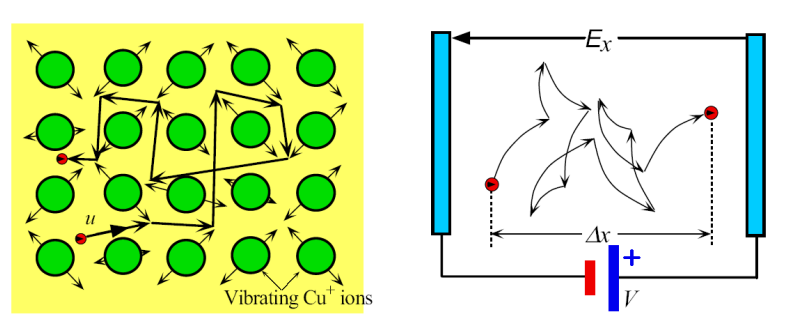
\includegraphics[width=0.99\linewidth]{Bilder/Drift}

\textbf{Elektrische Leitfähigkeit und Relaxationszeit (Stosszeit):}
\begin{equation*}
\sigma = \frac{n \cdot e^2 \cdot \tau}{m_e}
\end{equation*}

\textbf{Ladungsträgerdichte (aus makroskopischen Materialdaten):}
\begin{equation*}
n_{at} = \frac{\rho_m \cdot N_A}{M} \qquad \qquad Z = \frac{n}{n_{at}}
\end{equation*}

\begin{tabular}{@{}lll@{}}
    \toprule
    \textbf{Simbolo} & \textbf{Descrizione} & \textbf{Unità di Misura (SI)} \\
    \midrule
    $\sigma$ & Conducibilità elettrica & S/m (Siemens al metro) \\
    $n_{at}$ & Densità dei portatori di carica & $\text{m}^{-3}$ \\
    $\tau$ & Tempo di relax (Stosszeit) & s (secondi) \\
    $\rho_m$ & Densità di massa (Massendichte) & kg/$\text{m}^3$ \\
    $M$ & Massa Molare & kg/mol (o g/mol) \\
    $Z$ & Valenza (elettroni di conduzione per atomo) & adimensionale \\
    $N_A$ & Costante di Avogadro ($\approx 6.022 \cdot 10^{23}$) & $\text{mol}^{-1}$ \\
    \bottomrule
\end{tabular}

\subsection{Hall-Effekt(Hooool-Effekt)}
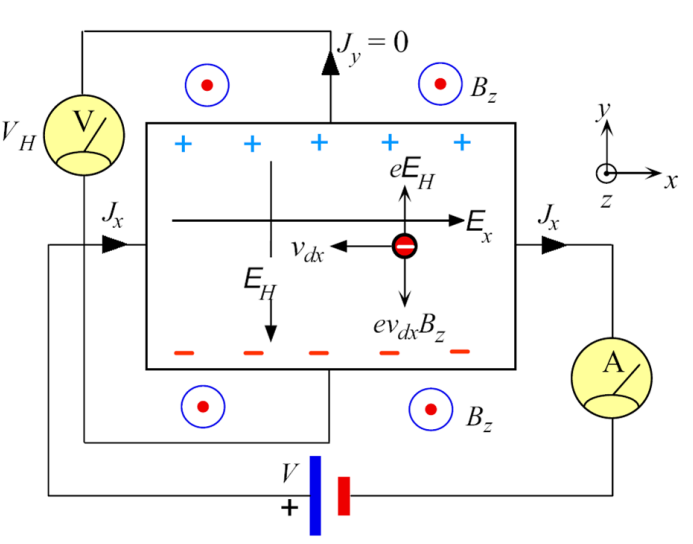
\includegraphics[width=0.97\linewidth]{Bilder/Halleffekt}
Ein Strom fliesst durch ein Stück leitendes Material, von links nach rechts(Bild). 
Ein magnetischer Fluss $B$ durchströmt das Material. Die Elektronen werden leicht abgelenkt und 
es entsteht ein weiteres Spannungspotential zwischen oben und unten, welches Hall-Spannung $V_H$ genannt wird.

\[R_H = - \frac{1}{e n} \qquad \mu = \sigma \cdot |R_H| \qquad \sigma =  n \cdot e \cdot \mu
\qquad U_H = \frac{I\cdot B \cos \alpha}{n \cdot e \cdot d}\]

\subsection{Skin-Effekt (Effetto Pelle)}
\begin{itemize}
    \item \textbf{Corrente Continua (DC):} La densità di corrente è distribuita in modo \textbf{omogeneo} su tutta la sezione trasversale del filo.
    \item \textbf{Corrente Alternata (AC):} La densità di corrente non è più uniforme. All'aumentare della frequenza, il flusso di corrente tende a concentrarsi verso la \textbf{superficie esterna} del conduttore.
\end{itemize}

\vspace{0.3cm}

La \textbf{profondità di penetrazione} (Skintiefe) $\delta$ indica lo spessore 
dello strato superficiale in cui scorre la maggior parte della corrente ed è definita 
dalla relazione:\vspace{-1em}

\[
\frac{1}{\delta} = \sqrt{\frac{1}{2}\sigma \mu_0 \mu_r \omega}
\]

\textbf{Legenda delle variabili:}
\begin{itemize}
    \item $\delta$: Profondità di penetrazione [m]
    \item $\sigma$: Conducibilità elettrica del materiale [S/m]
    \item $\mu_0$: Permeabilità magnetica del vuoto ($1.256 \times 10^{-6}$ H/m)
    \item $\mu_r$: Permeabilità relativa del materiale
    \item $\omega$: Frequenza angolare ($2\pi f$) [rad/s]
\end{itemize}

\subsection{Transporttherorie für Thermische Leitfähigkeit}
Elektrische Leiter sind (oft) auch gute thermische Leiter. 
Folglich tragen zu den Gitterschwingungen auch die freien Ladungsträger zum Wärmetransport bei.

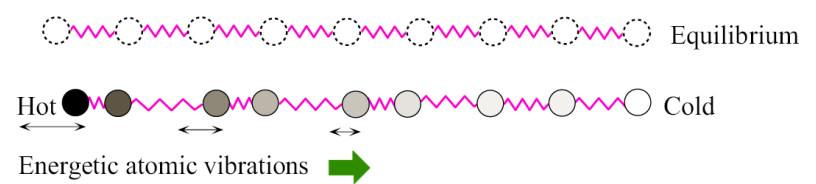
\includegraphics[width=0.85\linewidth]{Bilder/Thermische_Leitfähigkeit}

Eine höhere Kopplungsrate zwischen den Atomen führt zu einer schneller Übertragung von Gitterschwingungen. 
Somit sind mechanisch harte Materialien thermisch besser leitend als mechanisch weiche Materialien.\vspace{-1em}

\[\kappa = L \cdot \sigma \cdot T \qquad \text{dove } L = \frac{\pi^2 k_B^2}{3e^2} \approx 2.44 \cdot 10^{-8} \, \text{W}\Omega\text{K}^{-2} \qquad [T] = \kelvin\]